

\chapter{Functions}\label{chapter:functions}


In this chapter we explore general functions from tensors into other tensors.
While not quite as elegant as linear functions, they are important for many applications, such as non-linearities in neural networks.
The main goal is to make the vector chain rule intuitive and easy to apply, but we also cover Taylor series, determinants and other topics.

Standard notation for function over vectors can be quite ambiguous when the function broadcasts over some dimensions.
If $x\in\R^n$ is a vector, it's not clear whether $f(x)$ applies to each element of $x$ independently or if it's a function of the whole vector.
With tensor diagrams, we make this distinction clear by explicitly showing the edges of $x$ that go into $f$, and which don't.
We use the notation 
%If the result of $f(x)$ is itself a vector $\in\R^m$, we can write
\tikz[baseline=-.25em, inner sep=2pt]{
   \draw[->] (.5,0) node[right]{$x$} -- node[above, font=\tiny]{$n$} (0,0) node(f)[left]{$f$};
   \draw (f) -- ++(-.5,0) node[midway, above, font=\tiny] {$m$};
}
when $f$ is a function from $\R^n$ to $\R^m$.
If $f$ is element-wise, we write
$(\tikz[baseline=-.25em, inner sep=2pt]{
   \draw[->, densely dotted] (.3,0) node[right](x){$x$} -- (0,0) node(f)[left]{$f$};
   \draw (x) -- ++(.5,0) node[midway, above, font=\tiny] {$n$};
}) \in \R^n$.
We always assume that the function (arrow) edges are contracted before normal edges.
If we want something else, like $f(Mx)$, we can use brackets:
\tikz[baseline=(f.base), inner xsep=2pt, inner ysep=0pt]{
   \node (f) at (0,0) {$f$};
   \draw (f) -- ++(-.5,0);
   \node (group) at (1.5,0) {$(
      \tikz {
         \node (M) at (0.5,0) {$M$};%
         \draw (0,0) -- (M) -- ++(.5,0) node[right]{$x$};%
      }%
      )$
   };
   \draw[->] (group) -- (f);
}.
It may be helpful with some more examples:
%In the examples below, $x\in \R^n$:
\vspace{-1.5em}
\begin{center}
\begingroup
\renewcommand{\arraystretch}{2.5}
\begin{tabular}[h]{cccc}
   $f : \mathbb R^n \to \mathbb R$
   & $f(x) \in \mathbb R$
   & \tikz[baseline=-.25em]{\draw[->] (.5,0) node[right]{$x$} -- node[above, font=\tiny]{$n$} (0,0) node[left]{$f$}}
   & (Scalar function)
   \\
   $g : \mathbb R^n \to \mathbb R^m$
   & $g(x) \in \mathbb R^m$
   & \tikz[baseline=(x.base)]{
      \node (x) at (0,0) {$x$};
      \node (g) at (-.75,0) {$g$};
      \draw[->] (x) -- (g) node[midway, above, font=\tiny] {$n$};
      \draw (g) -- ++(-.5,0) node[midway, above, font=\tiny] {$m$};
   }
   & (Vector function)
   \\
   $h : \mathbb R \to \mathbb R$
   & $h(x) \in \mathbb R^n$
   & \tikz[baseline=(x.base)]{
      \node (x) at (0,0) {$x$};
      \node (h) at (-.75,0) {$h$};
      \draw[->, densely dotted] (x) -- (h);
      \draw (x) -- ++(.5,0) node[right, font=\tiny] {$n$};
   }
   & (Element-wise function)
   \\
   \makecell[c]{$u : \mathbb{R}^n \to \mathbb{R}^m$ \\ $v \in \mathbb{R}^m$}
   & $v^T u(x) \in \mathbb R$
   & \tikz[baseline=(x.base)]{
      \node (x) at (0,0) {$x$};
      \node (v) at (-.75,0) {$v$};
      \node (u) at (-1.5,0) {$u$};
      \draw[->] (x) -- (v) node[midway, above, font=\tiny] {$n$};
      \draw (v) -- (u) node[midway, above, font=\tiny] {$m$};
   }
   & (Vector times vector function)
   \\
   \makecell[c]{$A : \mathbb R^n \to \mathbb R^{m\times n},$\\$v \in \mathbb R^n$}
   & $A(x)v \in \mathbb R^m$
   & 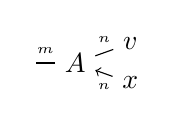
\begin{tikzpicture}[baseline=(A.base)]
      \node (A) at (0,0) {$A$};
      \draw (A) -- ++(-.5,0) node[midway, above, font=\tiny] {$m$};
      \node (x) at (.7,-.25) {$x$};
      \draw[->] (x) -- (A) node[midway, below, font=\tiny] {$n$};
      \node (v) at (.7,.25) {$v$};
      \draw (v) -- (A) node[midway, above, font=\tiny] {$n$};
   \end{tikzpicture}
   & (Vector times matrix function)
   \\
   \makecell[c]{$f : \mathbb R^d \to \mathbb R,$\\$X \in \mathbb R^{b\times d}$}
   & $f(X) \in \mathbb R^b$
   & 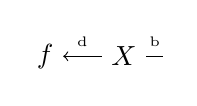
\begin{tikzpicture}[baseline=-.25em]
      \node (f) at (0,0) {$f$};
      \node (X) at (1,0) {$X$};
      \draw[->] (X) -- (f) node[midway, above, font=\tiny] {d};
      \draw (X) --  ++(.5,0) node[midway, above, font=\tiny] {b};
   \end{tikzpicture}
   & (Vector function, batched)
   \\
   \makecell[c]{$A : \mathbb R^{n\times m} \to \mathbb R,$\\$X \in \mathbb R^{n\times m}$}
   & $A(X) \in \R$
   & 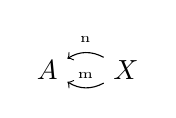
\begin{tikzpicture}[baseline=-.25em]
      \node (A) at (0,0) {$A$};
      \node (X) at (1,0) {$X$};
      \draw[->] (X) edge[bend right] node[midway, above, font=\tiny] {n} (A);
      \draw[->] (X) edge[bend left] node[midway, above, font=\tiny] {m} (A);
   \end{tikzpicture}
   & (Matrix input function)
   \\
   \makecell[c]{
      $f : \mathbb R^n\times \R^m \to \R^d$
      ,\\$u \in \mathbb R^{b\times n}
      , v \in \R^{b\times m}$
   }
   & $f(u, v) \in \R^{b \times d}$
   & 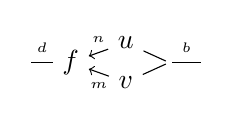
\begin{tikzpicture}[baseline=-.25em]
      \node (f) at (0,0) {$f$};
      \draw (f) -- ++(-.5,0) node[midway, above, font=\tiny] {$d$};
      \node (u) at (.7,.25) {$u$};
      \draw[->] (u) -- (f) node[midway, above, font=\tiny] {$n$};
      \node (v) at (.7,-.25) {$v$};
      \draw[->] (v) -- (f) node[midway, below, font=\tiny] {$m$};
      \node[inner sep=1pt] (d) at (1.25,0) {$\sbullet$};
      \draw (u) -- (d);
      \draw (v) -- (d);
      \draw (d) -- ++(.4,0) node[midway, above, font=\tiny] {$b$};
   \end{tikzpicture}
   & (Two inputs, batched)
\end{tabular}
\endgroup
\end{center}

To make it more concrete, let's consider some well known functions:
(1) The determinant function, $\det : \mathbb R^{n\times n} \to \mathbb R$ is a scalar function, and we can apply it to a batch of matrices by \tikz[baseline=(det.base), inner sep=2pt, every node/.append style={anchor=base}]{
      \node (det) {$\det$};
      \node[right=1.5em of det] (X) {$X$};
      \draw[->] (X) edge[bend right] node[midway, above, font=\tiny] {n} (det);
      \draw[->] (X) edge[bend left] node[midway, above, font=\tiny] {m} (det);
      \draw (X) -- ++(.5,0) node[right, font=\tiny] {$b$};
   } which results in a single vector $\in\R^b$.
%
   (2)
   Cosine similarity, $\mathrm{cossim} : \mathbb R^n \times \mathbb R^n \to \mathbb R$ is a scalar function, and we can apply it to two vectors by \tikz[baseline=(cos.base), inner sep=2pt, every node/.append style={anchor=base}]{
      \node (cos) at (0,0) {$\mathrm{cossim}$};
      \node (u) at (1,.15) {$u$};
      \draw[->] (u) -- (cos) node[midway, above, font=\tiny] {$n$};
      \node (v) at (1,-.15) {$v$};
      \draw[->] (v) -- (cos) node[midway, below, font=\tiny] {$n$};
   } which results in a single value $\in\R$.
% 
   (3)
  If the element-wise power function, $\mathrm{pow}_n : \mathbb R \to \mathbb R$
      is be applied to two vectors, they simplify under the Hadamard product:
      \[
         \begin{tikzpicture}[baseline=(s.base), inner sep=2pt, every node/.append style={anchor=base}]
            \node (pown) {$\mathrm{pow}_n$};
            \node[right=1em of pown] (u1) {$u$};
            \node[below=.5em of pown] (powm) {$\mathrm{pow}_m$};
            \node[below=.5em of u1] (u2) {$u$};
            \draw (u1) edge[->, densely dotted] (pown);
            \draw (u2) edge[->, densely dotted] (powm);
            \node (s) at (1.5, -.25) {$\sbullet$};
            \draw (u1) -- (s);
            \draw (u2) -- (s);
            \draw (s) -- ++(.5,0);
         \end{tikzpicture}
         =
         \begin{tikzpicture}[baseline=(pow.base), inner sep=2pt, every node/.append style={anchor=base}]
            \node (pow) {$\mathrm{pow}_{n+m}$};
            \node[right=1em of pow] (u) {$u$};
            \draw (u) edge[->, densely dotted] (pow);
            \draw (u) -- ++(.5,0);
         \end{tikzpicture}
      \]

For a more advanced example, consider the softmax function:
\tikz[baseline=(sm.base), inner sep=2pt, every node/.append style={anchor=base}]{
   \node (sm) {$\mathrm{softmax}$};
   \node[right=1em of sm] (x) {$x$};
   \draw[->] (x) -- (sm) node[midway, above, font=\tiny] {$d$};
   \draw (sm) -- ++(-1,0) node[midway, above, font=\tiny] {$d$};
}.
We can write this using elementary functions as:
\[
   \mathrm{softmax}(x)
   =
   \frac{\mathrm{exp}(x)}{\mathrm{sum}(\mathrm{exp}(x))}
   =
   \begin{tikzpicture}[baseline=-1em, every node/.append style={anchor=base}]
      \node (ex1) at (0,0) {$\mathrm{exp}$};
      \node (x1) at (1,0) {$x$};
      \draw (ex1) edge[<-, densely dotted] (x1);
      \draw (x1) -- ++(.5,0);
      % Second row
      \node (pow) at (-1,-.6) {$\mathrm{pow}_{-1}$};
      \node[right=1em of pow] (b1) {$($};
      \node[right=0em of b1] (exp2) {$\mathrm{exp}$};
      \node[right=1em of exp2] (x2) {$x$};
      \node[right=1em of x2, inner sep=1pt] (s) {$\sbullet$};
      \draw (x2) edge[->, densely dotted] (exp2);
      \draw (b1) edge[->, densely dotted] (pow);
      \draw (x2) -- (s);
      \node[right=0em of s] (b2) {$)$};
   \end{tikzpicture}
\]
It looks a bit complicated at first, but let us break it down step by step:
$(\tikz[baseline=(ex1.base), every node/.append style={anchor=base}]{
   \node (ex1) at (0,0) {$\mathrm{exp}$};
   \node (x1) at (1,0) {$x$};
   \draw (ex1) edge[<-, densely dotted] (x1);
   \draw (x1) -- ++(.5,0);
}) \in \R^n$ is the element-wise exponential function.
If we contract it with $\tikz[baseline=(s.base)] {
   \node[inner sep=1pt] (s) {$\sbullet$};
   \draw (s) -- ++(-.4,0);
}$, we get the sum $s=\sum_i \exp(x_i)$.
Finally, we apply $\mathrm{pow}_{-1}$ to $s$ and multiply it with the exponential function to get the softmax function.

One situation where things may get a bit confusing if the output tensor is contracted with the broadcasting edges of an input tensor.
But as long as we remember to contract the function edges first, things work out.
For example, for a function $f : \R^n \to \R$ and a matrix $x \in \R^{m \times n}$:
\[
   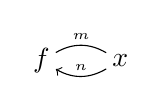
\begin{tikzpicture}[baseline=(f.base), inner sep=2pt]
      \node (f) {$f$};
      \node (x) at (1,0) {$x$};
      \draw (x) edge[bend right] node[midway, above, font=\tiny] {$m$} (f);
      \draw (x) edge[->, bend left] node[midway, above, font=\tiny] {$n$} (f);
   \end{tikzpicture}
   =
   \hspace{-2.3em}
   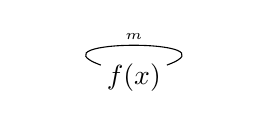
\begin{tikzpicture}[baseline=(f.base), inner sep=2pt]
      \node (f) {$f(x)$};
      \path (f) edge [out=160, in=20, looseness=3] node[midway, above, font=\tiny] {$m$} (f);
   \end{tikzpicture}
   \hspace{-2.3em}
   =
   \Tr(f(x))
   .
\]

\section{The Chain Rule}
One of the most attractive features of tensor diagrams is the transparency of the chain rule. For two functions
\(
   f: \mathbb{R}^m \to \mathbb{R} \quad \text{and} \quad v: \mathbb{R}^n \to \mathbb{R}^m,
\)
the composite function $f\circ v: \mathbb{R}^n \to \mathbb{R}$ is diagrammed simply by feeding the output of $v$ into $f$:
\[
   \tikz[baseline=(f.base), inner sep=2pt, every node/.append style={anchor=base}]{
      \node (f) {$f$};
      \node[right=1em of f] (v) {$v$};
      \node[right=1em of v] (x) {$x$};
      \draw[->] (x) -- (v);
      \draw[->] (v) -- (f);
   }
\]
In traditional notation, the chain rule is written
\(
   J_{f\circ v}(x)=\nabla f(v(x))\,J_v(x),
\)
where $J_v(x)$ is the Jacobian of $v$ and $\nabla f(v(x))$ is the gradient of $f$ at $v(x)$.
With tensor diagrams \emph{the chain rule is actually a chain!}
\[
   \begin{tikzpicture}[baseline=-1em, inner sep=1pt]
      \node (n0) {$f$};
      \node[below=1em of n0] (n1) {$v$};
      \node[below=1em of n1] (n2) {$x$};
      \draw[->] (n2) -- (n1);
      \draw[->] (n1) -- (n0);
      \drawellipse{0}{-.55}{.5}{1}{180/4}
   \end{tikzpicture}
   =
   \hspace{.5em}
   \begin{tikzpicture}[baseline=-1em, inner sep=1pt]
      \node[dn] (n0) {$f$};
      \node[below=1em of n0] (n1) {$v$};
      \node[below=1em of n1] (n2) {$x$};
      \node[right=1em of n0, dn] (n3) {$v$};
      \node[below=1em of n3] (n4) {$x$};
      \draw[->] (n2) -- (n1);
      \draw[->] (n1) -- (n0);
      \draw[->] (n4) -- (n3);
      \draw[d0] (n0) -- (n3);
      \draw[d0] (n3) -- ++(.5,0);
   \end{tikzpicture}
   \hspace{3em}
   \begin{tikzpicture}[baseline=-1em, inner sep=1pt]
      \node (n0) {$f$};
      \node[below=1em of n0] (n1) {$v$};
      \node[below=1em of n1] (n2) {$u$};
      \node[below=1em of n2] (n3) {$x$};
      \draw[->] (n3) -- (n2);
      \draw[->] (n2) -- (n1);
      \draw[->] (n1) -- (n0);
      \drawellipse{0}{-.75}{.5}{1.5}{180/4}
   \end{tikzpicture}
   =
   \hspace{.5em}
   \begin{tikzpicture}[baseline=-1em, inner sep=1pt]
      \node[dn] (n0) {$f$};
      \node[below=1em of n0] (n1) {$v$};
      \node[below=1em of n1] (n2) {$u$};
      \node[below=1em of n2] (n3) {$x$};
      \node[right=1em of n0] (n4) {$v$};
      \node[below=1em of n4] (n5) {$u$};
      \node[below=1em of n5] (n6) {$x$};
      \draw[->] (n3) -- (n2);
      \draw[->] (n2) -- (n1);
      \draw[->] (n1) -- (n0);
      \draw[->] (n6) -- (n5);
      \draw[->] (n5) -- (n4);
      \draw[d0] (n0) -- (n4);
      \drawellipse{.75}{-.55}{.5}{1}{180/4}
   \end{tikzpicture}
   =
   \hspace{.5em}
   \begin{tikzpicture}[baseline=-1em, inner sep=1pt]
      \node[dn] (n0) {$f$};
      \node[below=1em of n0] (n1) {$v$};
      \node[below=1em of n1] (n2) {$u$};
      \node[below=1em of n2] (n3) {$x$};
      \node[right=1em of n0, dn] (n4) {$v$};
      \node[below=1em of n4] (n5) {$u$};
      \node[below=1em of n5] (n6) {$x$};
      \node[right=1em of n4, dn] (n7) {$u$};
      \node[below=1em of n7] (n8) {$x$};
      \draw[->] (n3) -- (n2);
      \draw[->] (n2) -- (n1);
      \draw[->] (n1) -- (n0);
      \draw[->] (n6) -- (n5);
      \draw[->] (n5) -- (n4);
      \draw[->] (n8) -- (n7);
      \draw[d0] (n0) -- (n4);
      \draw[d0] (n4) -- (n7);
      \draw[d0] (n7) -- ++(.5,0);
   \end{tikzpicture}
\]
This clearly follows the classical mnemonic: ``the derivative of the outer function times the derivative of the inner function''.
The only refinement we need is that the ``outer function'' is connected to the ``inner function'' using the new edge created by taking the derivative.

We could further simplify \tikz[baseline=(f.base), inner sep=2pt]{\node[dn](f){$f$}; \draw[d0](f)--++(.6,0);} to \tikz[baseline=(f.base), inner sep=2pt]{\node(f){$f'$}; \draw(f)--++(.5,0);}, where $f'$ is the derivative of $f$.
For example, if $f$ was $\cos-$, then $f'$ would be $\sin-$.
But we can also just keep the circled $f$ as an easy to recognize symbol for the derivative.

\subsection{The Hessian Chain Rule}
Things get even more interesting when we consider the second derivative.
Using standard notation, the Hessian of $f\circ v$ is
\[
H_{f\circ v}(x) = Dv(x)^T \cdot D^2f(v(x)) \cdot Dv(x) + \sum_{k=1}^d \frac{\partial f}{\partial u_k}(v(x)) \frac{\partial^2 v_k}{\partial x \partial x^T}(x).
\]
This ``Hessian Chain Rule'' is much easier to derive using tensor diagrams:
\begin{align*}
   \begin{tikzpicture}[baseline=-1em, inner sep=1pt]
      \node (n0) {$f$};
      \node[below=1em of n0] (n1) {$v$};
      \node[below=1em of n1] (n2) {$x$};
      \draw[->] (n2) -- (n1);
      \draw[->] (n1) -- (n0);
      \drawellipse{0}{-.55}{.5}{1}{180/4}
      \drawellipse{0}{-.55}{.7}{1.2}{180/4}
   \end{tikzpicture}
   &=
   \hspace{.5em}
   \begin{tikzpicture}[baseline=-1em, inner sep=1pt]
      \node[dn] (n0) {$f$};
      \node[below=1em of n0] (n1) {$v$};
      \node[below=1em of n1] (n2) {$x$};
      \node[right=1em of n0, dn] (n3) {$v$};
      \node[below=1em of n3] (n4) {$x$};
      \draw[->] (n2) -- (n1);
      \draw[->] (n1) -- (n0);
      \draw[->] (n4) -- (n3);
      \draw[d0] (n0) -- (n3);
      \draw[d0] (n3) -- ++(.5,0);
      \drawellipse{.4}{-.55}{1}{1.2}{180/4}
   \end{tikzpicture}
 \\&=
   \hspace{.5em}
   \begin{tikzpicture}[baseline=-1em, inner sep=1pt]
      \node[dn] (n0) {$f$};
      \node[below=1em of n0] (n1) {$v$};
      \node[below=1em of n1] (n2) {$x$};
      \node[right=1.5em of n0, dn] (n3) {$v$};
      \node[below=1em of n3] (n4) {$x$};
      \draw[->] (n2) -- (n1);
      \draw[->] (n1) -- (n0);
      \draw[->] (n4) -- (n3);
      \draw[d0] (n0) -- (n3);
      \draw[d0] (n3) -- ++(.5,0);
      \drawellipse{0}{-.55}{.5}{1.2}{180/4}
   \end{tikzpicture}
   +
   \hspace{.5em}
   \begin{tikzpicture}[baseline=-1em, inner sep=1pt]
      \node[dn] (n0) {$f$};
      \node[below=1em of n0] (n1) {$v$};
      \node[below=1em of n1] (n2) {$x$};
      \node[right=1.5em of n0, dn] (n3) {$v$};
      \node[below=1em of n3] (n4) {$x$};
      \draw[->] (n2) -- (n1);
      \draw[->] (n1) -- (n0);
      \draw[->] (n4) -- (n3);
      \draw[d0] (n0) -- (n3);
      \draw[d0] (n3) -- ++(.5,0);
      \drawellipse{1}{-.25}{.5}{.7}{180/4}
   \end{tikzpicture}
 \\&=
   \hspace{.5em}
   \begin{tikzpicture}[baseline=-1em, inner sep=1pt]
      \node[ddn] (n0) {$f$};
      \node[below=1em of n0] (n1) {$v$};
      \node[below=1em of n1] (n2) {$x$};
      \node[right=1em of n0, yshift=-1em, dn] (n3) {$v$};
      \node[below=1em of n3] (n4) {$x$};
      \node[right=1.5em of n3, yshift=1em, dn] (n5) {$v$};
      \node[below=1em of n5] (n6) {$x$};
      \draw[->] (n2) -- (n1);
      \draw[->] (n1) -- (n0);
      \draw[->] (n4) -- (n3);
      \draw[->] (n6) -- (n5);
      \draw[d0] (n0) -- (n3);
      \draw[d0] (n0) -- (n5);
      \draw[d0] (n3) -- ++(.5,0);
      \draw[d0] (n5) -- ++(.5,0);
   \end{tikzpicture}
   +
   \hspace{.5em}
   \begin{tikzpicture}[baseline=-1em, inner sep=1pt]
      \node[dn] (n0) {$f$};
      \node[below=1em of n0] (n1) {$v$};
      \node[below=1em of n1] (n2) {$x$};
      \node[right=1.5em of n0, ddn] (n3) {$v$};
      \node[below=1em of n3] (n4) {$x$};
      \draw[->] (n2) -- (n1);
      \draw[->] (n1) -- (n0);
      \draw[->] (n4) -- (n3);
      \draw[d0] (n0) -- (n3);
      \draw[d0] (n3) -- ++(.5,0);
      \draw[d0] ($(n3)+(.166,.15)$) -- ++(.4,0);
   \end{tikzpicture}
\end{align*}
If we continue to expand this way, we see there is a simple pattern in the chain rule for more functions:
\[\makebox[\textwidth][c]{
   \begin{tikzpicture}[baseline=-1em, inner sep=1pt]
      \node (n0) {$f$};
      \node[below=1em of n0] (n1) {$v$};
      \node[below=1em of n1] (n2) {$u$};
      \node[below=1em of n2] (n3) {$x$};
      \draw[->] (n3) -- (n2);
      \draw[->] (n2) -- (n1);
      \draw[->] (n1) -- (n0);
      \drawellipse{0}{-.75}{.5}{1.4}{180/4}
      \drawellipse{0}{-.75}{.6}{1.5}{180/4}
   \end{tikzpicture}
   =
   \hspace{.2em}
   \begin{tikzpicture}[baseline=-1em, inner sep=1pt]
      \node[ddn] (n0) {$f$};
      \node[below=1em of n0] (n1) {$v$};
      \node[below=1em of n1] (n2) {$u$};
      \node[below=1em of n2] (n3) {$x$};
      \draw[->] (n3) -- (n2);
      \draw[->] (n2) -- (n1);
      \draw[->] (n1) -- (n0);
%
      \node[right=1em of n0, yshift=-1em, dn] (n4) {$v$};
      \draw[d0] (n0) -- (n4);
      \node[below=1em of n4] (n5) {$u$};
      \node[below=1em of n5] (n6) {$x$};
      \draw[->] (n6) -- (n5);
      \draw[->] (n5) -- (n4);
      \node[right=1em of n4, dn] (u1) {$u$};
      \node[below=1em of u1] (u2) {$x$};
      \draw[->] (u2) -- (u1);
      \draw[d0] (n4) -- (u1);
      \draw[d0] (u1) -- ++(.5,0);
%
      \node[right=3.5em of n4, yshift=1em, dn] (n7) {$v$};
      \draw[d0] (n0) -- (n7);
      \node[below=1em of n7] (n8) {$u$};
      \node[below=1em of n8] (n9) {$x$};
      \draw[->] (n9) -- (n8);
      \draw[->] (n8) -- (n7);
      \node[right=1em of n7, dn] (u3) {$u$};
      \node[below=1em of u3] (u4) {$x$};
      \draw[->] (u4) -- (u3);
      \draw[d0] (n7) -- (u3);
      \draw[d0] (u3) -- ++(.5,0);
   \end{tikzpicture}
   +
   \hspace{.2em}
   \begin{tikzpicture}[baseline=-1em, inner sep=1pt]
      \node[dn] (n0) {$f$};
      \node[below=1em of n0] (n1) {$v$};
      \node[below=1em of n1] (n2) {$u$};
      \node[below=1em of n2] (n3) {$x$};
      \node[right=1.5em of n0, ddn] (n4) {$v$};
      \node[below=1em of n4] (n5) {$u$};
      \node[below=1em of n5] (n6) {$x$};
      \draw[->] (n3) -- (n2);
      \draw[->] (n2) -- (n1);
      \draw[->] (n1) -- (n0);
      \draw[->] (n6) -- (n5);
      \draw[->] (n5) -- (n4);
      \draw[d0] (n0) -- (n4);
      %
      \node[right=1em of n4, yshift=-1em, dn] (r1) {$u$};
      \node[below=1em of r1] (r2) {$x$};
      \draw[->] (r2) -- (r1);
      %
      \node[right=1.5em of r1, yshift=1em, dn] (r3) {$u$};
      \node[below=1em of r3] (r4) {$x$};
      \draw[->] (r4) -- (r3);
      %
      \draw[d0] (n4) -- (r1);
      \draw[d0] (n4) -- (r3);
      \draw[d0] (r1) -- ++(.5,0);
      \draw[d0] ($(r3)+(.166,.15)$) -- ++(.4,0);
   \end{tikzpicture}
   +
   \hspace{.2em}
   \begin{tikzpicture}[baseline=-1em, inner sep=1pt]
      \node[dn] (n0) {$f$};
      \node[below=1em of n0] (n1) {$v$};
      \node[below=1em of n1] (n2) {$u$};
      \node[below=1em of n2] (n3) {$x$};
      \node[right=1.5em of n0, dn] (n4) {$v$};
      \node[below=1em of n4] (n5) {$u$};
      \node[below=1em of n5] (n6) {$x$};
      \node[right=1.5em of n4, ddn] (n7) {$u$};
      \node[below=1em of n7] (n8) {$x$};
      \draw[->] (n3) -- (n2);
      \draw[->] (n2) -- (n1);
      \draw[->] (n1) -- (n0);
      \draw[->] (n6) -- (n5);
      \draw[->] (n5) -- (n4);
      \draw[->] (n8) -- (n7);
      \draw[d0] (n0) -- (n4);
      \draw[d0] (n4) -- (n7);
      \draw[d0] (n7) -- ++(.5,0);
      \draw[d0] ($(n7)+(.166,.15)$) -- ++(.4,0);
   \end{tikzpicture}
}\]
Yaroslav Bulatov has written extensively on the Hessian Chain Rule, and how to evaluate it efficiently for deep learning applications.
Interested readers may refer to his blog post on the topic.

\subsection{Chain Rule with Broadcasting}
When the chain rule is applied to functions with broadcasting, the result still follows the ``outer derivative times inner derivative'' mnemonic, but the meaning of ``times'' is expanded to take the Hadamard product of the broadcasted edges.
\[
   \includegraphics[width=.8\textwidth]{figures/chain_rule_broadcast.pdf}
\]

\subsection{Functions with multiple inputs}
If $f : \mathbb{R}^m \times \mathbb{R}^n \to \mathbb{R}$ is a function with two inputs, the derivative of $f(x,y)$ is simply $\frac{\partial f}{\partial x}\partial x + \frac{\partial f}{\partial y}\partial y$,
or in tensor diagram notation:
\[
   \includegraphics[width=.45\textwidth]{figures/multi_input_functions.pdf}
\]

\section{Examples}

\subsection{Known derivatives}
Two examples where we can expand \tikz[baseline=(f.base), inner sep=2pt]{\node[dn](f){$f$}; \draw[d0](f)--++(.6,0);} with known derivatives:
\[
   \includegraphics[width=\textwidth]{figures/other_functions.pdf}
\]
Here $\mathrm{inv}(X)$ is the matrix inverse function, taking a matrix $X$ to its inverse $X^{-1}$.
In the case of the determinant, one may continue taking derivatives to find the
simple pattern
\[
   \frac{\partial^k \det(X)}{\partial X^k} = \det(X) (X^{-1})^{\otimes k}.
\]


\subsection{Pseudo-linear forms}

Pseudo-linear forms, $A(x)x$, are common.
All pixel-adaptive filters like non-local means, bilateral, etc, and the so-called attention mechanism in transformers can be written this way.
According to Peyman Milanfar, the gradient of this function is important and has a form worth remembering:
\[
   \begin{tikzpicture}[baseline=-1em, inner sep=1pt]
      \node (n0) {$A$};
      \node[below=1em of n0] (n1) {$x$};
      \node[right=1em of n0] (n2) {$x$};
      \draw[->] (n1) -- (n0);
      \draw (n2) -- (n0);
      \drawellipse{.25}{-.25}{.7}{.7}{180/4}
      \draw (n0) -- ++(-.5,0);
   \end{tikzpicture}
   =
   \hspace{.5em}
   \begin{tikzpicture}[baseline=-1em, inner sep=1pt]
      \node (n0) {$A$};
      \node[below=1em of n0] (n1) {$x$};
      \node[right=1em of n0] (n3) {$x$};
      \draw[->] (n1) -- (n0);
      \draw (n0) -- (n3);
      \drawellipse{0}{-.25}{.4}{.7}{180/4}
      \draw (n0) -- ++(-.5,0);
   \end{tikzpicture}
   +
   \hspace{.5em}
   \begin{tikzpicture}[baseline=-1em, inner sep=1pt]
      \node (n0) {$A$};
      \node[below=1em of n0] (n1) {$x$};
      \node[right=.75em of n0] (n3) {$x$};
      \draw[->] (n1) -- (n0);
      \draw (n0) -- (n3);
      \draw (n0) -- ++(-.5,0);
      \drawellipse{.575}{0}{.25}{.25}{180/4}
   \end{tikzpicture}
   =
   \hspace{.5em}
   \begin{tikzpicture}[baseline=-1em, inner sep=1pt]
      \node[dn] (n0) {$A$};
      \node[below=1em of n0] (n1) {$x$};
      \node[right=.75em of n0] (n3) {$x$};
      \draw[->] (n1) -- (n0);
      \draw (n0) -- (n3);
      \draw[d0] (n0) -- ++(.4,.4);
      \draw (n0) -- ++(-.5,0);
   \end{tikzpicture}
   +
   \hspace{.5em}
   \begin{tikzpicture}[baseline=-1em, inner sep=1pt]
      \node (n0) {$A$};
      \node[below=1em of n0] (n1) {$x$};
      \draw[->] (n1) -- (n0);
      \draw (n0) -- ++(.5,0);
      \draw (n0) -- ++(-.5,0);
   \end{tikzpicture}
\]
We may appreciate the simplicity of this expression, when we consider the following derivation given by Peyman Milanfar using classical notation:
\begin{align*}
   \mathrm{d}[A(x) x]
   & =\mathrm{d}[A(x)] x+A(x) \mathrm{d} x 
   \\& =\operatorname{vec}{\mathrm{d}[A(x)] x}+A(x) \mathrm{d} x 
   \\& =\operatorname{vec}{I \mathrm{d}[A(x)] x}+A(x) \mathrm{d} x 
   \\& =(x^T \otimes I) \operatorname{vec}{\mathrm{d}[A(x)]}+A(x) \mathrm{d} x 
   \\& =(x^T \otimes I) \mathrm{D} \operatorname{vec}[A(x)] \mathrm{d} x+A(x) \mathrm{d} x 
   \\& =[(x^T \otimes I) \mathrm{D} \operatorname{vec}[A(x)]+A(x)] \mathrm{d} x
\end{align*}
Which finally implies:
\begin{align*}
\hspace{-2em}
   \frac{\partial A(x)x}{\partial x}
   &= (x^T \otimes I) \frac{\partial}{\partial x}  \mathrm{vec}[A(x)] + A(x)
   .
\end{align*}

\subsection{Trace identity}
The Matrix Cookbook has the formula:
\begin{align}
   \tag{128}
   \frac{\partial \Tr(\sin(x))}{\partial x}
   &= \cos(x)^T
\end{align}
If we attempt to derive this using tensor diagrams, we get the following different result,
\[
   \includegraphics[width=.5\textwidth]{figures/cos.pdf}
\]
which is equivalent to $\cos(x) \circ I$.
That is, $\cos(x)$ but zero everywhere except the diagonal.

The reason is that the matrix cookbook actually uses a slightly different definition of ``function applied to matrix''.
If $F$ can be written as a power series, then one way to define $F(X)$ is the matrix power series:
\[
   F(X) = \sum_{k=0}^\infty a_k X^k.
\]
In this case, the derivative of $\Tr(F(X))$ is
$f(X)^T$, where $f(X)$ is the scalar derivative of $F(X)$,
matching the Matrix Cookbook's formula.


\subsection{Taylor}
For an n-times differentiable function $v: \R^d\to\R^d$ we can write the Taylor expansion:
\[
   \begin{tikzpicture}[baseline=-1em, inner sep=1pt]
      \node (n0) {$v$};
      \node[below=1em of n0] (n1) {$(x+\eps)$};
      \draw[->] (n1) -- (n0);
      \draw (n0) -- ++(.5,0);
   \end{tikzpicture}
   \approx
   \begin{tikzpicture}[baseline=-1em, inner sep=1pt]
      \node (n0) {$v$};
      \node[below=1em of n0] (n1) {$x$};
      \draw[->] (n1) -- (n0);
      \draw (n0) -- ++(.5,0);
   \end{tikzpicture}
   +
   \begin{tikzpicture}[baseline=-1em, inner sep=1pt]
      \node[dn] (n0) {$v$};
      \node[below=1em of n0] (n1) {$x$};
      \node[left=1em of n0] (n2) {$\eps$};
      \draw[->] (n1) -- (n0);
      \draw[d0] (n0) -- (n2);
      \draw (n0) -- ++(.5,0);
   \end{tikzpicture}
   +\frac12
   %\hspace{.5em}
   \begin{tikzpicture}[baseline=-1em, inner sep=1pt]
      \node[ddn] (n0) {$v$};
      \node[below=1em of n0] (n1) {$x$};
      \node[left=1em of n0] (n2) {$\eps$};
      \node[left=.75em of n0, yshift=-1em] (n3) {$\eps$};
      \draw[->] (n1) -- (n0);
      \draw[d0] (n0) -- (n2);
      \draw[d0] (n0) -- (n3);
      \draw (n0) -- ++(.5,0);
   \end{tikzpicture}
   +
   \frac16
   %\hspace{.5em}
   \begin{tikzpicture}[baseline=-1em, inner sep=1pt]
      \node[dddn] (n0) {$v$};
      \node[below=1em of n0] (n1) {$x$};
      \node[left=1em of n0] (n2) {$\eps$};
      \node[left=.75em of n0, yshift=-1em] (n3) {$\eps$};
      \node[left=.75em of n0, yshift=1em] (n4) {$\eps$};
      \draw[->] (n1) -- (n0);
      \draw[d0] (n0) -- (n2);
      \draw[d0] (n0) -- (n3);
      \draw[d0] (n0) -- (n4);
      \draw (n0) -- ++(.5,0);
   \end{tikzpicture}
   +
   \dots
\]

Writing this using classical notation is quite messy:
\begin{align*}
    v(x + \eps)
    &\approx
    v(x)
    + \left[\frac{\partial}{\partial x} v(x)\right]\eps
    + \frac{1}{2}\left[\frac{\partial}{\partial x}\left[\frac{\partial}{\partial x} v(x)\right]\eps\right]\eps
    + \frac{1}{6}\left[\frac{\partial}{\partial x}\left[\frac{\partial}{\partial x} \left[\frac{\partial}{\partial x} v(x)\right]\eps\right]\eps\right]\eps
    + \dots
    \\
    &=
    v(x)
    + \left[\frac{\partial}{\partial x} v(x)\right]\eps
    +
    \frac{1}{2}
    (I \otimes \eps)
    \left[\frac{\partial\mathrm{vec}}{\partial x}\left[\frac{\partial v(x)}{\partial x} \right]\right]\eps
    + \frac{1}{6}
    (I \otimes \eps \otimes \eps)
    \left[\frac{\partial\mathrm{vec}}{\partial x}\left[\frac{\partial\mathrm{vec}}{\partial x} \left[\frac{\partial v(x)}{\partial x} \right]\right]\right]\eps
    + \dots
\end{align*}
With index notation it's ok:
\begin{align*}
    v_i(x + \eps)
    &\approx
    v_i(x)
    + \sum_j \frac{\partial v_i(x)}{\partial x_j} \eps_j
    + \frac12 \sum_{j,k} \frac{\partial^2 v_i(x)}{\partial x_j\partial x_k} \eps_j \eps_k
   + \frac16 \sum_{j,k,\ell} \frac{\partial^3 v_i(x)}{\partial x_j\partial x_k\partial x_\ell} \eps_j \eps_k \eps_\ell
\end{align*}
% TODO: Examples based on idempotent matrices etc.



\section{Exercises}
\begin{exercise}
   Draw the tensor diagram for a function $f:\mathbb{R}^n\to\mathbb{R}$ that applies an element-wise nonlinearity (for instance, $\exp$) followed by a summation over the components. Verify that the diagram corresponds to the conventional formula for the softmax denominator.
\end{exercise}

\begin{exercise}
   Represent the composition of two functions 
   \[
      f:\mathbb{R}^m\to\mathbb{R} \quad \text{and} \quad v:\mathbb{R}^n\to\mathbb{R}^m,
   \]
   using tensor diagrams. Then, using the diagrammatic chain rule, derive the expression for the derivative of $f\circ v$ with respect to $x\in\mathbb{R}^n$.
\end{exercise}

\begin{exercise}
   For a matrix function $A(x)$ that depends on a vector $x$, use tensor diagrams to illustrate the derivative 
   \[
      \frac{\partial}{\partial x}[A(x)x],
   \]
   and explain how the product rule is implemented in the diagram.
\end{exercise}

\begin{exercise}
   % Source: Adapted from StackExchange VAE backpropagation questions (e.g., by greg).
   % Answer: Using the chain rule and elementwise differentiation, one obtains 
   % $\nabla_W KL = \frac{1}{2}\Big(e^{Wx+c} - 1\Big)x^T$, where the exponential is applied elementwise.
   Represent the KL-divergence term for a Variational Autoencoder (VAE) as
   \[
      KL(\mu,\sigma) = -\frac{1}{2}\Big(1 + \log\sigma^2 - \mu^2 - \sigma^2\Big),
   \]
   with parameters given by 
   \[
      \mu = W x + c \quad \text{and} \quad \log\sigma^2 = W x + c.
   \]
   Derive the gradient $\nabla_W KL$ with respect to the weight matrix $W$. Be sure to keep track of dimensions and account for elementwise operations.
\end{exercise}
\begin{exercise}
   % Source: A well-known result in machine learning; see many SE posts (e.g., greg's answers).
   % Answer: The Jacobian is given by 
   % $\displaystyle \frac{\partial s_i}{\partial z_j} = s_i\big(\delta_{ij} - s_j\big)$.
   Let the softmax function $s:\mathbb{R}^n \to \mathbb{R}^n$ be defined by
   \[
      s_i(z) = \frac{e^{z_i}}{\sum_{j=1}^n e^{z_j}}, \quad i=1,\dots,n.
   \]
   Prove that the Jacobian matrix of $s$ is given by
   \[
      \frac{\partial s_i}{\partial z_j} = s_i\big(\delta_{ij} - s_j\big),
   \]
   where $\delta_{ij}$ is the Kronecker delta.
\end{exercise}

\begin{exercise}
   % Source: Standard derivations found in textbooks and the Matrix Cookbook.
   % Answer: Differentiation yields $\nabla_\mu \ell = \Sigma^{-1}\sum_{i}(x^{(i)}-\mu)$ and 
   % $\nabla_\Sigma \ell = -\frac{n}{2}\Sigma^{-1} + \frac{1}{2}\Sigma^{-1}S\Sigma^{-1}$; setting these to zero leads to 
   % $\hat\mu = \frac{1}{n}\sum_{i=1}^n x^{(i)}$ and $\hat\Sigma = \frac{1}{n}\sum_{i=1}^n (x^{(i)}-\hat\mu)(x^{(i)}-\hat\mu)^T$.
   Suppose $x^{(1)},\dots,x^{(n)} \in \mathbb{R}^d$ are independent samples from a multivariate normal distribution $N(\mu,\Sigma)$. Write the log-likelihood function and derive the gradients $\nabla_\mu \ell$ and $\nabla_\Sigma \ell$. Then, by setting these gradients to zero, show that the maximum likelihood estimators are
   \[
      \hat\mu = \frac{1}{n}\sum_{i=1}^n x^{(i)} \quad \text{and} \quad \hat\Sigma = \frac{1}{n}\sum_{i=1}^n (x^{(i)} - \hat\mu)(x^{(i)} - \hat\mu)^T.
   \]
\end{exercise}

\begin{exercise}
   % Source: Derived from Gaussian process literature and related SE discussions.
   % Answer: The derivative is 
   % $\displaystyle \frac{\partial L}{\partial \theta} = \frac{1}{2}\operatorname{tr}\!\Big(\Big(K^{-1}yy^T K^{-1} - K^{-1}\Big)\frac{\partial K}{\partial \theta}\Big)$.
   Consider a Gaussian process with covariance matrix $K(\theta)$ and the log-marginal likelihood defined as
   \[
      L(\theta) = -\frac{1}{2}\Big(y^T K(\theta)^{-1} y + \log\det K(\theta)\Big).
   \]
   Derive the gradient of $L$ with respect to $\theta$, showing that
   \[
      \frac{\partial L}{\partial \theta} = \frac{1}{2}\operatorname{tr}\!\Big(\Big(K^{-1}yy^T K^{-1} - K^{-1}\Big)\frac{\partial K}{\partial \theta}\Big).
   \]
\end{exercise}

\begin{exercise}
   % Source: Standard logistic regression derivations and multiple SE posts.
   % Answer: One obtains $\nabla_w J = \sum_{i=1}^n (p_i - y_i)x_i$ and the Hessian 
   % $H = \sum_{i=1}^n p_i(1-p_i)x_i x_i^T$.
   In logistic regression, let 
   \[
      p_i = \sigma(w^T x_i) \quad \text{with} \quad \sigma(z)=\frac{1}{1+e^{-z}},
   \]
   and consider the negative log-likelihood
   \[
      J(w) = -\sum_{i=1}^n \Big[y_i\ln p_i + (1-y_i)\ln(1-p_i)\Big].
   \]
   Derive the gradient $\nabla_w J$ and the Hessian $H = \nabla^2_w J$. In particular, show that
   \[
      \nabla_w J = \sum_{i=1}^n (p_i - y_i)x_i, \quad \text{and} \quad H = \sum_{i=1}^n p_i(1-p_i)\,x_i x_i^T.
   \]
\end{exercise}

\begin{exercise}
   % Source: Matrix Cookbook and classic derivations in matrix calculus.
   % Answer: The derivative is $\nabla_X \det(X) = \det(X)\,(X^{-1})^T$.
   Let $X \in \mathbb{R}^{n\times n}$ be an invertible matrix. Prove that
   \[
      \frac{\partial\,\det(X)}{\partial X} = \det(X)\,(X^{-1})^T.
   \]
   In other words, show that the gradient of $\det(X)$ with respect to $X$ is $\det(X)$ times the transpose of $X^{-1}$.
\end{exercise}

\begin{exercise}
   % Source: Standard result from the Matrix Cookbook.
   % Answer: $\nabla_X \ln\det(X) = (X^{-1})^T$.
   For an invertible matrix $X \in \mathbb{R}^{n\times n}$, prove that
   \[
      \frac{\partial}{\partial X}\ln\det(X) = (X^{-1})^T.
   \]
   Briefly discuss why this result is useful in statistical applications such as Gaussian likelihoods.
\end{exercise}

\begin{exercise}
   % Source: Matrix Cookbook and related SE discussions.
   % Answer: By differentiating $I = A^{-1}A$, we find 
   % $d(A^{-1}) = -A^{-1}(dA)A^{-1}$.
   Let $A \in \mathbb{R}^{n\times n}$ be an invertible matrix (which may depend on a parameter). Starting from the identity $I = A^{-1}A$, differentiate both sides to show that
   \[
      d(A^{-1}) = -A^{-1}\,(dA)\,A^{-1}.
   \]
   Deduce an expression for the partial derivative $\frac{\partial A^{-1}}{\partial A_{ij}}$.
\end{exercise}

\begin{exercise}
   % Source: Derived from the differentiation of an inverse matrix (see Matrix Cookbook).
   % Answer: The gradient is given by 
   % $\nabla_A f(A) = -A^{-T}(a\,b^T)A^{-T}$.
   Define the scalar function
   \[
      f(A)=a^T A^{-1} b,
   \]
   where $a,b\in\mathbb{R}^n$ are fixed vectors and $A\in\mathbb{R}^{n\times n}$ is invertible. Using the result from differentiating the inverse, show that
   \[
      \nabla_A f(A) = -A^{-T}(a\,b^T)A^{-T}.
   \]
\end{exercise}

\begin{exercise}
   % Source: A classical perturbation result found in textbooks and SE posts.
   % Answer: For a simple eigenvalue $\lambda$ with unit eigenvector $v$, 
   % $\nabla_X \lambda = v\,v^T$. This result does not hold when $\lambda$ is multiple.
   Let $X\in\mathbb{R}^{n\times n}$ be a symmetric matrix with a simple eigenvalue $\lambda$ and corresponding unit eigenvector $v$. Prove that the derivative of $\lambda$ with respect to $X$ is given by
   \[
      \nabla_X \lambda = v\,v^T.
   \]
   Additionally, discuss why this result does not hold when $\lambda$ has multiplicity greater than one.
\end{exercise}

\begin{exercise}
   % Source: Classical result using Lagrange multipliers; see standard textbooks.
   % Answer: The stationary condition yields $Ax = \lambda x$, so the extrema of the Rayleigh quotient are the eigenvalues of $A$, with the maximizer (minimizer) corresponding to the largest (smallest) eigenvalue.
   For a symmetric matrix $A\in\mathbb{R}^{n\times n}$, consider the Rayleigh quotient
   \[
      R(x) = \frac{x^T A x}{x^T x}, \quad x\in\mathbb{R}^n\setminus\{0\}.
   \]
   Using Lagrange multipliers, show that the stationary values of $R(x)$ correspond to the eigenvalues of $A$, and that the maximizer (minimizer) is the eigenvector associated with the largest (smallest) eigenvalue.
\end{exercise}
\begin{exercise}
   % Source: Matrix Cookbook and common SE answers.
   % Answer: The derivative is 
   % $\nabla_X\,\operatorname{Tr}(X^T A X B) = A X B^T + A^T X B$.
   Let $A\in\mathbb{R}^{m\times m}$ and $B\in\mathbb{R}^{n\times n}$ be constant matrices, and let $X\in\mathbb{R}^{m\times n}$ be a variable matrix. Prove that
   \[
      \nabla_X\,\operatorname{Tr}(X^T A X B) = A X B^T + A^T X B.
   \]
   (Hint: Use the cyclic property of the trace to rearrange terms.)
\end{exercise}

\begin{exercise}
   % Source: Direct differentiation of trace forms; see also the Matrix Cookbook.
   % Answer: (a) $\frac{\partial}{\partial X} \operatorname{Tr}(A^T X) = A$, (b) $\nabla_X\,\operatorname{Tr}(A X B) = A^T B^T$.
   \textbf{(a)} Show that for a constant matrix $A\in\mathbb{R}^{m\times n}$ and variable $X\in\mathbb{R}^{m\times n}$,
   \[
      \frac{\partial}{\partial X} \operatorname{Tr}(A^T X) = A.
   \]
   \textbf{(b)} More generally, for constant matrices $A\in\mathbb{R}^{p\times m}$ and $B\in\mathbb{R}^{n\times q}$, prove that
   \[
      \nabla_X\,\operatorname{Tr}(A X B) = A^T B^T.
   \]
\end{exercise}

\begin{exercise}
   % Source: Inspired by tensor diagram techniques and SE discussions.
   % Answer: By differentiating $F(s)=\Diag(s)C\Diag(s)$, one obtains 
   % $dF = \Diag(ds)C\,\Diag(s) + \Diag(s)C\,\Diag(ds)$, leading to 
   % $\nabla_s F(s)$ that relates (after suitable vectorization) to $2\,\Diag(C\,s)$.
   Let $s\in\mathbb{R}^n$ be a vector and $C\in\mathbb{R}^{n\times n}$ be a fixed matrix. Define the matrix function 
   \[
      F(s) = \diag(s)\,C\,\diag(s),
   \]
   where $\diag(s)$ denotes the diagonal matrix with the entries of $s$. Express the differential $dF$ in terms of $s$, $ds$, and $C$, and hence derive an expression for the derivative $\nabla_s F(s)$.
\end{exercise}

\begin{exercise}
   % Source: Standard vectorization identities from the Matrix Cookbook.
   % Answer: The identity is 
   % $\operatorname{vec}(A\,X\,B^T) = (B \otimes A)\,\operatorname{vec}(X)$.
   Let $A\in\mathbb{R}^{p\times m}$, $X\in\mathbb{R}^{m\times n}$, and $B\in\mathbb{R}^{n\times q}$. Prove the identity
   \[
      \operatorname{vec}(A\,X\,B^T) = (B \otimes A)\,\operatorname{vec}(X).
   \]
   Discuss how this identity can be used to convert certain matrix derivative problems into vectorized forms.
\end{exercise}
\begin{exercise}
   % Source: Standard differentiation of quadratic forms.
   % Answer: The gradient is $\nabla_x f(x) = (A+A^T)x$, and the Hessian is $\nabla^2_x f(x) = A+A^T$. For symmetric $A$, this simplifies to $2A$.
   Let 
   \[
      f(x) = x^T A x,
   \]
   where $x\in\mathbb{R}^n$ and $A\in\mathbb{R}^{n\times n}$ is not necessarily symmetric. Show that
   \[
      \nabla_x f(x) = (A + A^T)x.
   \]
   Then, compute the Hessian $\nabla^2_x f(x)$ and discuss what simplification occurs when $A$ is symmetric.
\end{exercise}
\begin{exercise}
   % Source: Standard convex analysis and properties of the Frobenius norm.
   % Answer: For $X\neq 0$, $\nabla_X \|X\|_F = \frac{X}{\|X\|_F}$. At $X=0$, the gradient is not unique; any matrix $G$ with $\|G\|_F\le 1$ is a subgradient.
   Consider the Frobenius norm
   \(
      \|X\|_F = \sqrt{\operatorname{Tr}(X^T X)},
   \)
   for $X\in\mathbb{R}^{m\times n}$.

   Show that
   \[
      \nabla_X \|X\|_F = \frac{X}{\|X\|_F}
   \]
   for $X\neq 0$.
\end{exercise}
\begin{exercise}
   % Source: Based on discussions of spectral function differentiability on SE.
   % Answer: When the largest eigenvalue has multiplicity $k>1$, any matrix of the form 
   % $G = \sum_{i=1}^k u_i v_i^T$, where $\{u_i\}$ is an orthonormal basis for the eigenspace, is a valid subgradient. The gradient is not unique in this case.
   Let $Y\in\mathbb{R}^{n\times n}$ be a symmetric matrix, and define $\phi(Y)$ to be its largest eigenvalue. If this eigenvalue has multiplicity $k>1$, show that the derivative of $\phi(Y)$ is not unique. In particular, demonstrate that any matrix of the form
   \[
      G = \sum_{i=1}^k u_i v_i^T,
   \]
   where $\{u_i\}_{i=1}^k$ is any orthonormal basis for the eigenspace corresponding to the largest eigenvalue, is a valid subgradient of $\phi(Y)$. Explain the challenges that arise in defining a unique gradient in this setting.
\end{exercise}
